\chapter{Zastosowane technologie}
\label{cha:teoria}
Niniejszy rozdział zawiera krótki opis najważniejszych technologii i narzędzi używanych przez autorów podczas pracy z oprogramowaniem systemu GGSS. Przedstawione tu opisy zawierają podstawową wiedzę o sposobie działania i użytkowania tych technologii - szczegółowe przykłady przedstawione zostały w dalszej części pracy, w kontekście konkretnych rozwiązań zrealizowanych przez autorów w projekcie.


\section{Język C++}
\textit{C++} jest kompilowanym językiem programowania ogólnego przeznaczenia \cite{Bjarne} opartym o statyczne typowanie. Został stworzony jako obiektowe rozszerzenie języka C (z którym jest w dużej mierze wstecznie kompatybilny), lecz wraz z rozwojem pojawiło się w nim wsparcie dla innych paradygmatów, w tym generycznego i funkcyjnego. Sprawiło to, że język ten stał się bardzo wszechstronny - pozwala zarówno na szybkie wykonywanie operacji niskopoziomowych, jak i na tworzenie wysokopoziomowych abstrakcji \cite{Bjarne}. Dodatkową cechą wyróżniającą C++ wśród innych języków umożliwiających programowanie obiektowe jest jego wysoka wydajność.

\paragraph*{Standardy języka}\mbox{} \\
W ciągu ostatnich kilku lat C++ przechodzi proces intensywnego rozwoju - od 2011 roku pojawiły się trzy nowe standardy tego języka, a kolejny przewidziany jest na rok 2020. Wspomniane nowe standardy to:
\begin{itemize}
\item C++11 - wprowadza funkcjonalności takie jak: wsparcie dla wielowątkowości, wyrażenia lambda, referencje do \textit{r-wartości}, biblioteka do obsługi wyrażeń regularnych, dedukcja typów za pomocą słowa kluczowego \textit{auto} czy pętla zakresowa. Standard ten uważany jest za przełom w rozwoju języka.
\item C++14 - rozszerza zmiany wprowadzone w C++11. Nie zawiera tak wielu przełomowych zmian jak poprzedni standard - twórcy skupili się na poprawie istniejących błędów oraz rozwoju istniejących rozwiązań \cite{Cpp14Wikipedia}, np. dedukcji typu zwracanego z funkcji za pomocą słowa kluczowego \textit{auto}.
\item C++17 - wprowadza m.in. nowe typy danych (np. \textit{std::variant}, \textit{std::byte} i \textit{std::optional}), algorytmy współbieżne, biblioteka \textit{filesystem} przeznaczona do obsługi systemu plików oraz rozszerzenie mechanizmu dedukcji typów w szablonach na szablony klas \cite{BartekCodingBlogCpp17}. Standard ten usuwa również pewne elementy uznane za przestarzałe, np. inteligentny wskaźnik \textit{std::auto\_ptr}, zastąpiony w standardzie C++11 przez inne rozwiązanie.
\end{itemize} 
Zmiany wprowadzane w nowych standardach pozwalają na tworzenie czytelniejszego kodu, który łatwiej utrzymywać i rozwijać. Ma to znaczenie zarówno na poziomie pojedynczych instrukcji czy typów danych, jak i na poziomie architektury projektu. Listingi \ref{lst:cpp03} oraz \ref{lst:cpp11} przedstawiają przykład zmiany, jaka zaszła między starym standardem C++03, a C++11. Zaprezentowany kod realizuje w obu przypadkach iterację po zawartości kontenera typu \textit{std::vector<int>} mającą na celu wypisanie na standardowe wyjście jego zawartości. Przykład ten, pomimo że bardzo prosty, dobrze obrazuje wzrost jakości i czytelności kodu w nowym standardzie.

\begin{lstlisting}[language=c++,caption={Przykład kodu w języku C++ napisany z wykorzystaniem standardu C++03},label={lst:cpp03}]
// kontener zawierający 6 elementów typu int - inicjalizacja
// za pomocą tymczasowej tablicy, możliwa w statym standardzie
// języka
int tmp_arr[] = {1, 2, 3, 4, 5, 6};
std::vector<int> a (tmp_arr, tmp_arr + 6);

// iteracja po zawartości kontenera w standardzie C++03
for (std::vector<int>::const_iterator it = a.begin(); it != a.end(); ++it) {
    std::cout << *it << " ";
}
\end{lstlisting}

\begin{lstlisting}[language=c++,caption={Przykład kodu w języku C++ napisany z wykorzystaniem funkcjonalności ze standardu C++11 (zakresowa pętla for)},label={lst:cpp11}]
// kontener zawierający 6 elementów typu int - nowy
// sposób inicjalizacji
std::vector<int> a{1, 2, 3, 4, 5, 6};

// iteracja po zawartości kontenera w standardzie C++11 - 
// przykład zastosowania zakresowej pętli for
for (const auto& elem: a) {
	std::cout << elem << " ";
}
\end{lstlisting}


\paragraph*{Boost}\mbox{} \\
\textit{Boost} jest zestawem bibliotek dla języka C++, poszerzających w znacznym stopniu wachlarz narzędzi programistycznych dostarczanych przez język. Biblioteki wchodzące w skład Boost dostarczają funkcjonalności takich, jak: wygodne przetwarzanie tekstu, zapewnienie interfejsu między C++ a językiem Python czy programowanie sieciowe \cite{BoostDocs}. Boost to projekt aktywnie rozwijany, bardzo popularny. Niektóre z bibliotek wchodzących w jego skład zostały przeniesione (nie zawsze w postaci identycznej względem oryginału) do standardu C++.

\section{Biblioteki}
Biblioteki są jedym z podstawowych narzędzi wprowadzających podział programu na niezależne komponenty oraz dających możliwość wielokrotnego użycia tego samego kodu. Stanowią więc zbiór funkcji, struktur itp. udostępnionych do użycia przez inne programy. Niniejsza część pracy skupia się na bibliotekach opisywanych z perspektywy języków C oraz C++. Opis dotyczył będzie rozwiązań związanych z systemami typu UNIX (nie zostanie poruszony sposób działania bibliotek na systemach Windows). Autorzy zdecydowali się opisać to zagadnienie szczegółowo z uwagi na fakt, iż architektura projektu GGSS w dużej mierze opiera się o mechanizm bibliotek. Rozważania teoretyczne wzbogacone zostaną więc prostym przykładem.

\paragraph*{Opis przykładu}\mbox{}\\
Przykład prezentujący działanie bibliotek został napisany w języku C i  składa się z dwóch katalogów: \textit{app}, zawierającego kod źródłowy programu, oraz \textit{complex}, zawierającego kod źródłowy, który zostanie wykorzystany do stworzenia prostej biblioteki pozwalającej na wykonywanie podstawowych operacji na liczbach zespolonych. Listing \ref{lst:libexample} zawiera wynik polecenia \textit{tree}, które wypisuje na standardowe wyjście strukturę katalogu z projektem. Autorzy zdecydowali się pokazać proces budowania bibliotek bez wykorzystania narzędzi automatyzujących ten proces (takich jak \textit{CMake}), gdyż znajomość zasad działania tego mechanizmu okazała się dla nich bardzo pomocna podczas rozwiązywania problemów związanych z wykorzystaniem bibliotek w systemie GGSS, gdzie wspomniane narzędzia były już używane.

\begin{lstlisting}[language=bash, caption={Struktura katalogów projektu stanowiącego bazę przykładu dotyczącego bibliotek.},label={lst:libexample}]
user@host:~$ tree --charset=ascii
.
|-- app
|   `-- app.c
`-- complex
    |-- complex_number.h
    |-- complex_opers.c
    `-- complex_opers.h

2 directories, 4 files
\end{lstlisting}

\subsection{Rodzaje bibliotek}
Na systemach z rodziny UNIX wyróżniamy dwa podstawowy typy bibliotek: \textbf{statyczne} oraz \textbf{współdzielone (shared)}, nazywane również \textbf{dynamicznymi}. Podejścia te znacznie różnią się od siebie. Każde z nich oferuje pewne zalety względem drugiego, przez co oba pozostają dziś w użyciu.

\subsection{Biblioteki statyczne}
Koncepcja stojąca za bibliotekami statycznymi jest bardzo prosta - są to archiwa zawierające w sobie kolekcję plików obiektowych (\textit{*.o}). Do tego typu bibliotek dołączone muszą być pliki nagłówkowe zawierające m.in. deklaracje funkcji stanowiących interfejs pomiędzy biblioteką, a używającym ją programem. Cechą bibliotek statycznych odróźniającą je od bibliotek dynamicznych jest fakt, że są one dołączane do plików obiektowych głównego programu w czasie linkowania - stanowią więc część wynikowego pliku wykonywalnego. 



\paragraph*{Tworzenie biblioteki statycznej}\mbox{}\\
Rysunek \ref{fig:staticlibflow} przedstawia schematycznie proces tworzenia bibliotek statycznych. Składa się on z dwóch etapów:
\begin{itemize}
\item kompilacja plików źródłowych biblioteki do postaci obiektowej za pomocą \textit{gcc} (listing \ref{lst:libstat1}). Wynikiem powinny być pliki o rozszerzeniu \textit{*.o} odpowiadające wykorzystanym plikom źródłowym.

\begin{lstlisting}[language=bash, caption={Kompilacja plików źródłowych biblioteki do postaci obiektowej - polecenie oraz jego wynik},label={lst:libstat1}]
user@host:~/complex$ gcc -c *.c
user@host:~/complex$ ls
complex_number.h  complex_opers.c  complex_opers.h  complex_opers.o
\end{lstlisting}


\item utworzenie archiwum zawierającego pliki obiektowe za pomocą programu \textit{archiver} (listing \ref{lst:libstat2}). Wynikiem powinien być plik o rozszerzeniu \textit{*.a}. Podczas tworzenia biblioteki należy nadać jej odpowiednią nazwę, zgodną z formatem \textit{lib<nazwa>.a}.

\begin{lstlisting}[language=bash, caption={Utworzenie biblioteki statycznej z plików obiektowych - polecenie oraz jego wynik},label={lst:libstat2}]
user@host:~/complex$ ar -rc libcoml.a *.o
user@host:~/complex$ ls
complex_number.h  complex_opers.c  complex_opers.h  complex_opers.o  libcoml.a
\end{lstlisting}

\end{itemize}

\begin{figure}%[H]
\centering
\caption{Proces tworzenia biblioteki statycznej z uwzględnieniem komend koniecznych do wykonania poszczególnych etapów}
\label{fig:staticlibflow}
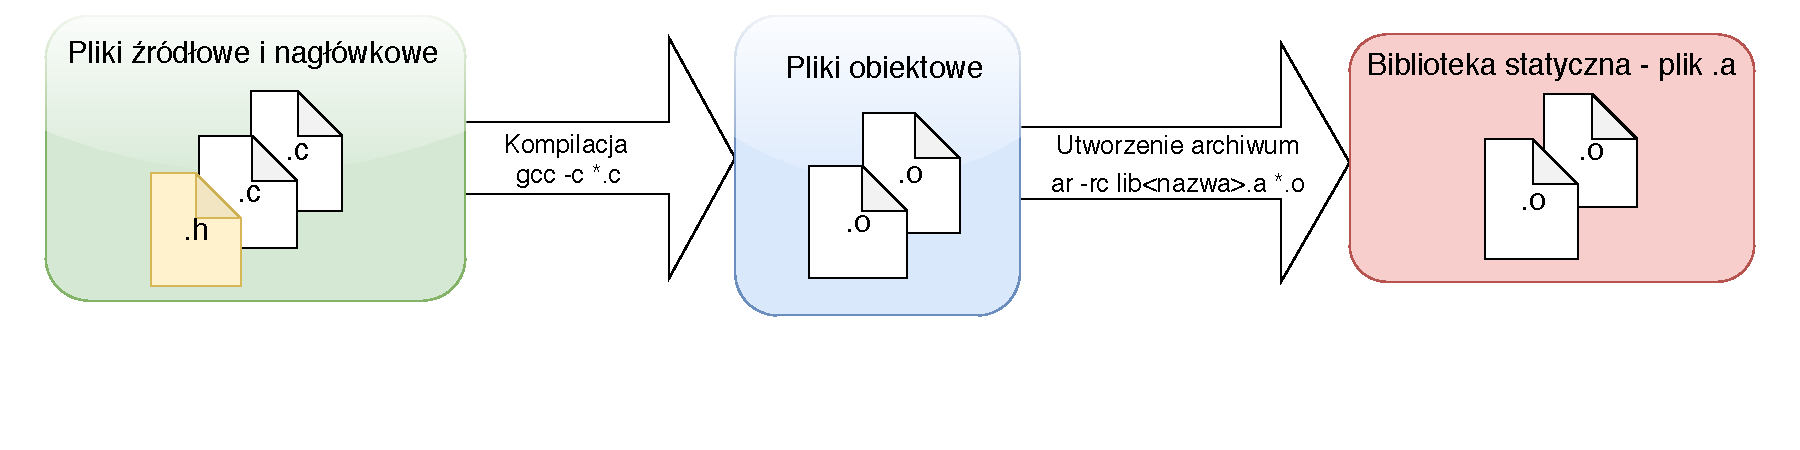
\includegraphics[width=\textwidth]{res/StaticLibFlow}
\end{figure}

Zawartość powstałego archiwum można zbadać za pomocą komendy \textit{ar -t} - wyświetla ona wszyskie pliki obiektowe wchodzące w skład danej biblioteki. Istnieje również możliwość wylistowania symboli - służy do tego narzędzie \textit{nm}. Użycie tych narzędzi na wykonanym przez autorów przykładzie ilustruje listing \ref{lst:libstat3}. Wynikiem polecenia \textit{nm} są tam dwa symbole, oznaczające dwie udostępnione dla użytkowników biblioteki funkcje (dodawanie i odejmowanie liczb zespolonych).

\begin{lstlisting}[language=bash, caption={Użycie poleceń \textit{ar -t} oraz \textit{nm} na bibliotece statycznej.},label={lst:libstat3}]
user@host:~/complex$ ar -t libcoml.a
complex_opers.o
user@host:~/complex$ nm libcoml.a

complex_opers.o:
0000000000000000 T add_complex_numbers
0000000000000091 T subtract_complex_numbers
\end{lstlisting}


\paragraph*{Dołączanie utworzonej biblioteki do programu}\mbox{}\\
Rysunek \ref{fig:staticliblink} przedstawia schematycznie proces dołączania utworzonej biblioteki statycznej do programu. Proces ten składa się z następujących etapów:

\begin{figure}[H]
\centering
\caption{Proces dołączania biblioteki statycznej do programu z uwzględnieniem komend koniecznych do wykonania poszczególnych etapów}
\label{fig:staticliblink}
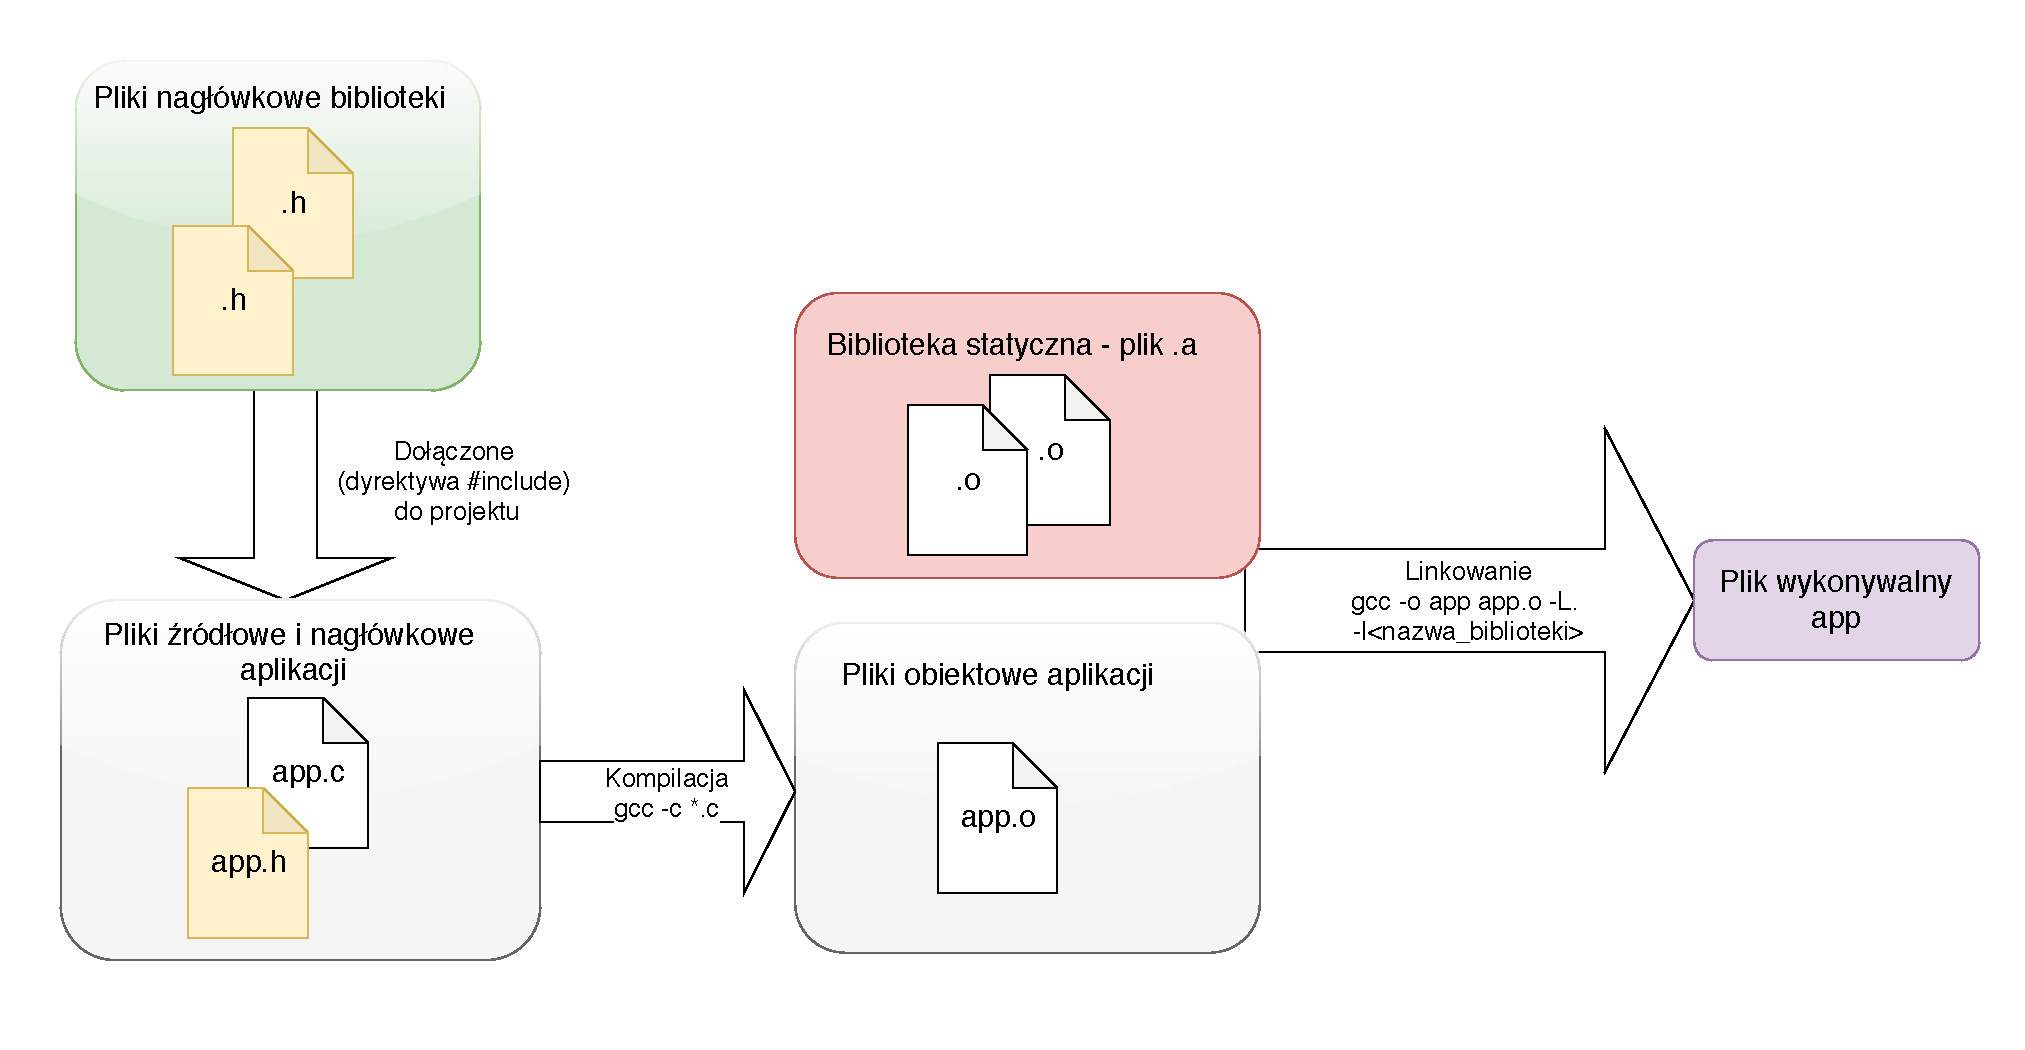
\includegraphics[width=\textwidth]{res/StaticLibLink}
\end{figure}

\begin{itemize}
\item dołączenie do źródeł programu plików nagłówkowych zawierających deklaracje stanowiące interfejs między programem a biblioteką (dyrektywa \textit{include} - listing \ref{lst:libstat4}).

\begin{lstlisting}[language=c++, caption={Plik \textit{app.c} zawierający dyrektywę \textit{include} dołączającą plik nagłówkowy zawierający deklaracje funkcji z biblioteki statycznej},label={lst:libstat4}]
#include "../complex/complex_opers.h"
#include <stdio.h>

int main(void) {

    complex_number a = {2.5, 3.7};
    complex_number b = {3.5, 0};

    complex_number c = add_complex_numbers(a, b);
    complex_number d = subtract_complex_numbers(a, b);

    printf("%lf %lf\n", c.real, c.imaginary);
    printf("%lf %lf\n", d.real, d.imaginary);

    return 0;
}
\end{lstlisting}

\item kompilacja plików źródlowych programu do postaci plików obiektowych za pomoca \textit{gcc} (listing \ref{lst:libstat5}). Wynikiem powinien być zestaw plików obiektowych odpowiadający wykorzystanym plikom źródłowym.

\begin{lstlisting}[language=bash, caption={Kompilacja plików źródłowych głównego programu do postaci obiektowej.},label={lst:libstat5}]
user@host:~/app$ gcc -c *.c
user@host:~/app$ ls
app.c  app.o
\end{lstlisting}


\item połączenie plików obiektowych i biblioteki w plik wykonywalny za pomocą \textit{gcc} (listing \ref{lst:libstat6}). Opcja \textit{-L} pozwala określić ścieżkę do dołączanej biblioteki, natomiast \textit{-l} - nazwę bibliteki (bez przedrostka \textit{lib} i rozszerzenie \textit{.a}).

\begin{lstlisting}[language=bash, caption={Linkowanie plików obiektowych programu z biblioteką statyczną, wynik uruchomienia programu obrazuący poprawne działanie przykładu.},label={lst:libstat6}]
user@host:~/app$ gcc -o app app.o -L../complex -lcoml
user@host:~/app$ ls
app  app.c  app.o
user@host:~/app$ ./app
6.000000 3.700000
-1.000000 3.700000
\end{lstlisting}

\end{itemize}

\subsection{Biblioteki współdzielone}



\paragraph*{Tworzenie biblioteki współdzielonej}\mbox{}\\
\paragraph*{Dołączanie utworzonej biblioteki do programu}\mbox{}\\
\paragraph*{Wersjonowanie bibliotek współdzielonych}

\subsection{Porównanie rodzajów bibliotek}

\section{Narzędzie CMake}

\textit{CMake (Cross-platform Make)} to narzędzie pozwalające na konfigurację procesu budowania oprogramowania (aplikacji oraz bibliotek) w sposób niezależny od platformy. Jego działanie opiera się na generowaniu pliku budującego natywnego dla określonej platformy \cite{CMakeIntro} (dla systemów z rodziny UNIX jest nim \textit{Makefile}) na podstawie przygotowanego przez użytkownika pliku \textit{CMakeLists.txt}. Takie podejście w znacznym stopniu ułatwia tworzenie aplikacji multiplatformowych oraz pozwala na intuicyjne zarządzanie zależnościami w projekcie. Domyślnie CMake pracuje z językami C i C++, natomiast nowe wersje narzędzia wpierają ponadto m.in. język C\# czy technologię CUDA \cite{CMakeSupport}. Narzędzie to jest rozwijane i wspierane przez firmę \textit{Kitware}.\par

\paragraph*{Plik CMakeLists.txt}\mbox{} \\
Jak wspomniano wyżej działanie narzędzia CMake opiera się na przygotowanym przez użytkownika pliku (lub zestawie plików rozmieszczonych w strukturze katalogów projektu) \textit{CMakeLists.txt}. Plik ten zawiera polecenia napisane w specjalnie do tego celu przygotowanym języku skryptowym. Użytkownik może za jego pomocą  m.in. określać jakie pliki wykonywalne mają zostać wygenerowane podczas procesu budowania, wskazać lokalizację plików źródłowych czy określić zależności między komponentami projektu oraz bibliotekami zewnętrznymi. \par

\paragraph*{Prosty przykład}\mbox{} \\
Listing \ref{lst:hello} zawiera przykład prostego pliku \textit{CMakeLists.txt}, pozwalającego na zbudowanie napisanej w języku C++ obiektowej wersji klasycznego programu \textit{Hello world}. Przykład ilustruje zastosowanie podstawowych poleceń CMake do określenia minimalnej wersji narzędzia, standardu języka C++, wynikowego pliku wykonywalnego oraz potrzebnych plików nagłówkowych. \par

\begin{lstlisting}[language=bash,caption={Przykład prostego pliku CMakeLists.txt przeznaczonego do budowania programu napisanego w C++}, label={lst:hello}]
# Określenie minimalnej wersji CMake
cmake_minimum_required(VERSION 3.0 FATAL_ERROR)

# Określenie standardu języka C++
set(CMAKE_CXX_STANDARD 14)
set(CMAKE_CXX_STANDARD_REQUIRED True)

# Nazwa oraz wersja projektu
project(Hello VERSION 1.0)

# Dodanie pliku wykonywalnego, który powinien powstać
# wskutek procesu budowania
add_executable(Hello Main.cpp)

# Dodanie do projektu katalogu include wraz ze znajdującym się 
# wewnątrz niego plikiem nagłówkowym
target_include_directories(Hello PUBLIC "${CMAKE_CURRENT_SOURCE_DIR}/include")
\end{lstlisting}

\paragraph*{Wersje CMake}\mbox{} \\
CMake jest narzedziem, który w ciągu ostatnich kilku lat przechodzi gruntowne zmiany. Starsze wersje (np. 2.8) oparte są o prosty system zmiennych \cite{CMakeRight}, co wprowadza szereg trudności w zarządzaniu dużymi projektami z wielopoziomowymi drzewami zależności. Dodatkowym problemem tych wersji jest również brak dobrze zdefiniowanych tzw. \textit{dobrych praktyk} oraz nieprzystępna dla początkujących dokumentacja. Współczesne wersje narzędzie CMake (zwykle za takie uznaje się nowsze od wersji 3.0) opierają się na innym, bardziej ustrukturyzowanym \cite{CMakeRight} podejściu, co było przyczyną pojawienia się dla nich wyżej wspomnianych \textit{dobrych praktyk}. Zalecane jest więc, by nowe projekty prowadzone były właśnie z użyciem nowszych wersji narzędzia.

\paragraph*{Narzędzia CTest i CPack}\mbox{} \\
CMake oferuje również możliwość konfiguracji sposobu testowania projektu. Służy do tego narzędzie \textit{CTest}, dystrybuowane razem z podstawowym narzędziem CMake. Innym przydatnym modułem jest \textit{CPack} - narzędzie to służy przygotowywaniu pakietów instalacyjnych z oprogramowaniem. Użycie obu wymienionych narzędzi polega na umieszczeniu w pliku \textit{CMakeLists.txt} kilku przeznaczonych do tego komend. \par 


\section{Język Python}
\textit{Python} jest nowoczesnym, wysokopoziomowym językiem programowania, wspierającym takie paradygmaty jak programowanie obiektowe czy imperatywne. Działanie Pythona opiera się na dynamicznym systemie typów. Z założenia Python jest językiem przyjemnym w użytkowaniu, co przyczyniło się do jego dużej popularności \cite{Lutz}. Python jest szeroko stosowany jako język skryptowy - takie też zastosowanie znalazł w projekcie GGSS.

\paragraph*{Prosty przykład}\mbox{} \\
Listing \ref{lst:pyexample} przedstawia prosty przykład skryptu napisanego w języku Python w wersji 3. Kod ten stanowi uproszczoną wersję skryptu zaprezentowanego w dalszej części pracy, którego zadaniem jest zbudowanie aplikacji w zależności od przekazanych przez użytkownika argumentów. Przykład prezentuje prosty skrypt przyjmujący jeden z dwóch możliwych argumentów i wypisujący informację na temat otrzymanego argumentu na standardowe wyjście.

\begin{lstlisting}[language=python,caption={Przykład prostego skryptu napisanego w języku Python 3 - przetwarzanie argumentów podanych przez użytkownika do skryptu}, label={lst:pyexample}]
import argparse

## Prosty skrypt przetwarzający argumenty podane 
## przy jego uruchomieniu przez użytkownika

## Definicja funkcji w języku Python
def parse_command_line_arguments():

    ## Obiekt przetwarzający argumenty (parser)
    parser = argparse.ArgumentParser()

    ## Argumenty wzajemnie się wykluczające
    group = parser.add_mutually_exclusive_group(required=True)
    group.add_argument("-s", "--staticboost", 
        help="Use static Boost linking.", action="store_true")
    group.add_argument("-d", "--dynamicboost",
        help="Use dynamic Boost linking.", action="store_true")

    return parser.parse_args()

if __name__=="__main__":
    ## Wywołanie funkcji
    arguments = parse_command_line_arguments()
    print(arguments)


\end{lstlisting}

\paragraph*{Wersje języka Python}\mbox{} \\
Python funkcjonuje w dwóch wersjach: Python 2 oraz 3. Wersje te nie są ze sobą w pełni kompatybilne, tzn. pewne funkcjonalności Pythona 2 nie są dostępne w Pythonie 3 i odwrotnie. Różnice znaleźć można również np. w domyślnym sposobie kodowania łańcuchów znakowych (ASCII w Pythonie 2, Unicode w Pythonie 3) oraz w wyniku dzielenia (za pomocą operatora \textit{/}) dwóch liczb całkowitych (w Pythonie 2 wynikiem jest liczba całkowita, w Pythonie 3 liczba zmiennoprzecinkowa typu \textit{float}) \cite{Python2vs3}. Ponadto zakończenie oficjalnego wsparcia Pythona w wersji 2 przewidziane jest na styczeń 2020 roku \cite{Python2Countdown} - co w momencie pisania niniejszej pracy (grudzień 2019) jest terminem niedalekim i miało kluczowe znaczenie w czasie podejmowania pewnych decyzji projektowych.

\paragraph*{Zewnętrzne biblioteki}\mbox{} \\
Jedną z największych zalet Pythona jest bardzo duża liczba bibliotek zewnętrznych tworzonych przez społeczność Pythona. Rozbudowują one język o wiele nowych funkcjonalności, np. przetwarzanie plików HTML czy wykonywanie obliczeń numerycznych. W niniejszej pracy zastosowanych zostało kilka tego typu bibliotek, m.in. \textit{Beautiful Soup} do wspomnianego wyżej przetwarzania dokumentów w formacie HTML. Omówienie ich działania na przykładach znaleźć można w dalszej części pracy - przy opisie konkretnego ich zastosowania. 


\section{Powłoka systemu operacyjnego - Bash}
Powłoka systemu jest programem, którego głównym zadaniem jest udostępnienie interfejsu umożliwiającego łatwy dostęp do funkcji systemu operacyjnego. Nazwę \textit{powłoka} zawdzięcza temu, że jest warstwą okalającą system operacyjny. Najczęściej spotykanym rodzajem powłoki są tzw. interfejsy z wierszem poleceń (ang. command-line interface). Polecenia wprowadzane są do nich w modzie interaktywnym, tj. wykonywane są one w momencie wprowadzenia końca linii.

\begin{lstlisting}[language=bash,caption={Komenda wypisująca tekst na standardowe wyjście wykonana z linii poleceń}]
user@host:~$ echo "interfejs z linią poleceń"
interfejs z linią poleceń
user@host:~$
\end{lstlisting}

Bash, czyli \textbf{Bourne Again Shell} jest powłoką systemu początkowo napisaną dla systemu operacyjnego GNU. Obecnie Bash jest kompatybilny z większością systemów Unixowych, gdzie zwykle jest powłoką domyślną oraz posiada kilka portów na inne platformy, tj.: MS-DOS, OS/2, Windows \cite{BashMan}. Oprócz pełnienia wyżej wymienionej funkcji, Bash jest również językiem programowania pozwalającym na tworzenie skryptów, które są kolejną metodą wprowadzania poleceń do powłoki systemu.\par
Korzystając z języka skryptowego powłoki Bash jesteśmy w stanie zawrzeć dodatkową logikę podczas wykonywania komend. Wspiera on takie struktury jak: instrukcje warunkowe, pętle, operacje logiczne oraz arytmetyczne. Aby wykorzystać Bash w skrypcie należy na początku pliku zamieścić zapis \textbf{\#!/bin/bash}, gdzie \textbf{/bin/bash} to ścieżka do pliku interpretera Bash. Zachowanie skryptu jesteśmy w stanie uzależnić od argumentów wykonania. Ich obsługa odbywa się za pomocą zapisu \textbf{\$?}, gdzie \textbf{?} jest to numer porządkowy argumentu liczony od 0.

\begin{lstlisting}[label={lst:prostySkrypt},language=bash,caption={Skrypt wykorzystujący argumenty wejściowe, instrukcję warunkową oraz polecenie echo}]
#!/bin/bash
if [ $1 == "argumenty" ]; then
        echo "Argument 0.: $0"
        echo "Argument 1.: $1"
else
        echo "Nieznane polecenie"
fi
\end{lstlisting}

\begin{lstlisting}[language=bash,caption={Przykład działania Skryptu z Listingu \ref{lst:prostySkrypt}}]
user@host:~$ /home/user/prostySkrypt.sh argumenty
Argument 0.: /home/user/prostySkrypt.sh
Argument 1.: argumenty
\end{lstlisting}

Bash posiada wiele poleceń, które pozwalają na wykonywanie zarówno podstawowych, jak i bardziej zaawansowanych czynności, np.: obsługa plików, obsługa systemu katalogów, zarządzanie kontami, uprawnieniami, itd.\par
Bash posiada również wiele zaawansowanych funkcjonalności, które pozwalają na kontrolowanie przepływu informacji w trakcie wykonywania poleceń. Przykładem jest wpisywanie tekstu do pliku ukazane na Listingu \ref{lis:zapisDoPliku}.

\begin{lstlisting}[label={lis:zapisDoPliku},language=bash,caption={Przykład zapisu tekstu do pliku}]
user@host:~$ echo "Ten napis zostanie zapisany do pliku plik.txt" > plik.txt
user@host:~$ cat plik.txt
Ten napis zostanie zapisany do pliku plik.txt
\end{lstlisting}

W celu zapisania tekstu do pliku należy na standardowe wyjście przekazać napis za pomocą komendy \textbf{echo}, a następnie przekierować za pomocą zapisu \textbf{>}, który poprzedza nazwę pliku docelowego. W wyniku działania zawartośc pliku \textbf{plik.txt} zostanie nadpisana, a w przypadku gdy takiego pliku nie ma, to zostanie on utworzony i uzupełniony o napis.\par


\section{System kontroli wersji Git i portal Gitlab}
System kontroli wersji Git jest oprogramowaniem służącym do śledzenia i zarządzania zmianami w plikach projektowych. W przypadku Git'a, aby zarejestrować pliki projektowe w celu ich śledzenia należy wykonać kilka czynności. Po pierwsze wymagane jest utworzenie repozytorium. Sprowadza się ono do wykonania odpowiedniej komendy Git'a wewnątrz folderu projektu, tj. \textbf{git init}. Podczas działania komendy wewnątrz folderu, w którym wywołaliśmy ww. polecenie, inicjowany jest ukryty folder \textbf{.git}
. Jest on odpowiedzialny za przechowywanie konfiguracji dla tego repozytorium oraz zapisywanie informacji o wszystkich zmianach dokonanych w projekcie.

\begin{lstlisting}[language=bash,caption={Inicjalizacja repozytorium git}]
user@host:/ścieżka/do/projektu$ git init
Initialized empty Git repository in /ściezka/do/projektu
user@host:/ściezka/do/projektu$ ls .git
branches  config  description  HEAD  hooks  info  objects  refs
\end{lstlisting}

Taka inicjalizacja nie spowoduje żadnego dodatkowego działania oprócz utworzenia repozytorium. Żadne pliki nie są jeszcze poddawane rewizji. W celu rejestracji plików należy wykonać jeszcze kilka kroków. Pierwszym z nich jest wykonanie komendy \textbf{git add}, która poprzedza nazwę plików lub folderów, które chcemy poddać wersjonowaniu. Elementy te zostają dodane do tzw. poczekalni, czyli są one kandydatami do utworzenia kolejnej rewizji. Przydatną komendą w tym przypadku jest również \textbf{git status} pozwalająca na sprawdzenie obecnego stanu repozytorium. Wyświetla ono krótkie podsumowanie nt. nowych plików, usuniętych plików oraz plików zmodyfikowanych. Informuje nas również o tym, które pliki są brane pod uwagę do utworzenia kolejnej rewizji.

\begin{lstlisting}[language=bash,caption={Dodawanie elementów do poczekalni}]
user@host:/ściezka/do/projektu# git add plik1 folder1
user@host:/ściezka/do/projektu# git status
On branch master

No commits yet

Changes to be committed:
  (use "git rm --cached <file>..." to unstage)

        new file:   folder1/plik3
        new file:   folder1/plik4
        new file:   plik1

Untracked files:
  (use "git add <file>..." to include in what will be committed)

        plik2
\end{lstlisting}

\begin{figure}[H]
\centering
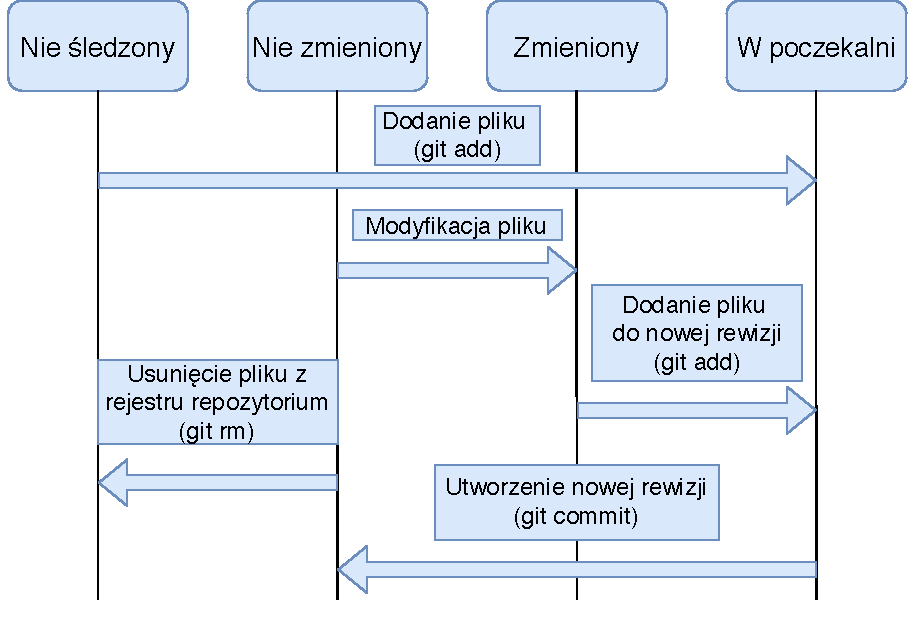
\includegraphics[width=0.8\textwidth]{res/fileStates.pdf}
\caption{Możliwe stany pliku w repozytorium GIT WSTAWIC REFERENCJE DO TEGO} 
\end{figure}

Tworzenie nowej wersji w ramach repozytorium odbywa się za pomocą komendy \textbf{git commit}. Sprowadza się do 'zamrożenia' obecnych wersji plików zarejestrowanych do rewizji oraz przypisanie im wspólnego, unikalnego dla każdej z nich, identyfikatora. Git udostępnia komendy pozwalające na przeglądanie oraz przywracanie plików do wcześniej utworzonych wersji. Listing \ref{lis:pierwszaRewizja} przedstawia utworzenie nowej wersji oraz wyświetlenie podsumowania o utworzonych do tej pory rewizjach.

\begin{lstlisting}[label={lis:pierwszaRewizja}, language=bash,caption={Utworzenie nowej rewizji}]
user@host:/sciezka/do/projektu# git commit -m "Pierwsza rewizja"
user@host:/sciezka/do/projektu# git log 
commit 1d2445e961beb25940dffa9d73963f887ee553ad
Author: user <user@host.localdomain>
Date:   Wed Dec 4 17:29:55 2019 +0100

    Pierwsza rewizja
\end{lstlisting}

Przejścia między rewizjami nie powodują utraty danych, gdyż zachowywana jest informacja o stanie plików dla każdej z nich, co ukazuje Listing \ref{lis:drugaRewizja}. Tworzona jest nowa rewizja zawierająca dodatkowo \textbf{plik2}, natomiast po powrocie do poprzedniej wersji plik ten nie występuje. Gdy powrócimy do nowszej wersji ponownie pojawi się \textbf{plik2}.

\begin{lstlisting}[language=bash,caption={Podsumowanie rewizji, powrót do starszej wersji},label={lis:drugaRewizja}]
user@host:/sciezka/do/projektu# git add plik2
user@host:/sciezka/do/projektu# git commit -m "Druga rewizja"
user@host:/sciezka/do/projektu# git log 
commit b58836df55fc2a8eb2a43aa96273853776924807
Author: user <user@host.localdomain>
Date:   Wed Dec 4 17:30:10 2019 +0100

    Druga rewizja

commit 1d2445e961beb25940dffa9d73963f887ee553ad
Author: user <user@host.localdomain>
Date:   Wed Dec 4 17:29:55 2019 +0100

    Pierwsza rewizja

user@host:/sciezka/do/projektu# ls
folder1  plik1  plik2
user@host:/sciezka/do/projektu# git checkout 1d2445e961beb25940dffa9d73963f887ee553ad
user@host:/sciezka/do/projektu# ls
folder1  plik1
user@host:/sciezka/do/projektu# git checkout b58836df55fc2a8eb2a43aa96273853776924807
user@host:/sciezka/do/projektu# ls
folder1  plik1  plik2
\end{lstlisting}

Głównym celem portalu \textbf{GitLab} jest udostępnienie środowiska do przechowywania repozytoriów Gitowych na zdalnych serwerach. Pozwala to na uniezależnienie się od maszyny na której pracujemy, zwiększa bezpieczeństwo plików źródłowych poprzez umieszczenie kopii na zdalnym serwerze oraz wspiera zespołową pracę nad kodem.\par

Ze względu na to, że portale typu \textbf{GitLab} są traktowane jako podstawowe narzędzie do wspólnej pracy nad kodem, to rozwinęły one wiele narzędzi wspomagających organizację oraz śledzenie pracy.Oprócz ww. funkcji \textbf{Gitlab} dostarcza wiele narzędzi do wspomagania procesu zapewniania jakości, jak i automatyzacji dostarczania kodu.\par

\textbf{Git} posiada specjalne komendy pozwalające na przekazywanie oraz pobieranie repozytoriów z ww. portali, czyli:
\begin{itemize}
\item \textbf{git clone}, która pozwala na pobranie repozytorium z portalu oraz zainicjalizowanie go lokalnie
\item \textbf{git pull} - za pomocą tej komendy możemy zaktualizować repozytorium lokalne do najnowszej rewizji, która znajduje się na portalu
\item oraz komenda \textbf{git push} aktualizująca zdalne repozytorium do naszej wersji
\end{itemize}

Jest to tylko podstawowy opis technologii jaką jest \textbf{Git}, przykłady bardziej zaawansowanych zastosowań pojawią się w części manuskryptu przeznaczonej na prezentację wykonanych prac w ramach projektu.


\section{Manager pakietów - RPM}
Menadżer pakietów jest zbiorem oprogramowania, które w sposób automatyczny zarządza instalacją, aktualizacją, konfiguracją oraz usuwaniem programów komputerowych \cite{ManagerWiki}. Ze względu na to, że procesy te różnią się w zależności od systemów operacyjnych oraz ich dystrybucji istnieje wiele menadżerów pakietów.\par

Zastosowanie technologii zarządzania pakietami pozwala znacząco zmniejszyć próg wejścia wynikający z użycia wcześniej niewykorzystywanego oprogramowania. Pozwala on odejść od żmudnego procesu ręcznej instalacji zależności oraz konfiguracji środowiska. Dzięki manadżerom wszystko jest wykonywane automatycznie. Jeżeli w trakcie procedur nie wystąpi żaden problem, to pakiet, którego zleciliśmy instalacje, powinien być od razu gotowy do działania. Jeżeli domyślna konfiguracja, jaka zostanie nam zapewniona w podczas działania menadżera pakietów, nie będzie dla nas odpowiednia możemy dokonać jej modyfikacji po procesie instalacji.

\newpage
RPM, czyli RedHat Package Manager jest darmowym, open-source'owym menadżerem pakietów dla systemów z rodziny RedHat oraz SUSE, czyli m.in.:
\begin{itemize}
\item RedHat Linux
\item CentOS
\item Fedora
\item openSUSE
\end{itemize}\par
RPM jest domyślnym manadżerem pakietów dla ww. dystrybucji. Obsługuje on pakiety w ramach formatu \textbf{.rpm}. Pakiety \textbf{.rpm} zawierają w sobie wiele ważnych elementów. Po pierwsze wewnątrz nich przechowywane są dane aplikacji, czyli: pliki wykonywalne, dokumentacja, testy, konfiguracja.\par 
Kolejnym ważnym elementem są informacje o zależnościach, czyli innych wymaganych pakietach, które pozwalają na automatyzację procesu instalacji. W momencie, gdy któraś z zależności jest niespełniona menadżer pakietów stara się odnaleźć, w bazie danych pakietów, odpowiedni wpis, aby \textbf{pobrać} oraz \textbf{zainstalować} brakujące oprogramowanie. Trzecim ważnym elementem jest logika pakietu, która jest podstawą do realizacji akcji wykonywanych przez menadżer pakietów, dostarczona w postaci skryptów powłoki, np. \textbf{bash}, zaszytych wewnątrz pliku *.rpm.

Listing \ref{lst:zawRPM} pokazuje przykładową zawartość pakietu, czyli moduł kernela \textbf{modułAplikacji}, plik w formacie \textbf{JSON} pozwalający na konfigurację aplikacji oraz plik wykonywalny \textbf{aplikacji}, natomiast  listing \ref{lis:skryptRPM} pokazuje przykładową logikę pakietu RPM w postaci skryptów shell. Skrypty te nie zawierają ani kopiowania, ani usuwania plików zawartych pakiecie, proces ten odbuwa się automatycznie na podstawie ścieżek ukazanych na Listingu \ref{lis:zawRPM} w trakcie instalacji/dezinstalacji.

\begin{lstlisting}[language=bash,caption={Przykładowa zawartość pakietu RPM},label={lst:zawRPM}]
user@host:~# rpm -qpl pakiet.rpm
/ścieżka
/ścieżka/do
/ścieżka/do/konfiguracjaAplikacji.json
/ścieżka/do/aplikacji
/usr
/usr/lib
/usr/lib/modules
/usr/lib/modules/3.10.0-862
/usr/lib/modules/3.10.0-862/extra
/usr/lib/modules/3.10.0-862/extra/modułAplikacji.ko
\end{lstlisting}

\newpage

\begin{lstlisting}[label={lis:skryptRPM}, language=bash, caption={Skrypty pakietu RPM}]
user@host:~# rpm -qp --scripts pakiet.rpm
preinstall program: /bin/sh
postinstall scriptlet (using /bin/sh):

#!/bin/sh
echo "Post-instajacja przykładowego pakietu"
echo "Przypisywanie uprawnień"
chmod 777 /ścieżka/do/konfiguracjaAplikacji.json
echo "Ładowanie modułu aplikacji"
/sbin/modrpobe modułAplikacji

preuninstall scriptlet (using /bin/sh):
#!/bin/sh
echo "Odinstalowywanie przykładowego pakietu"
echo "Usuwanie modułu aplikacji"
/sbin/rmmod modułAplikacji

postuninstall program: /bin/sh
\end{lstlisting}

\section{Technologie wirtualizacji i konteneryzacji}

\textbf{Wirtualizacja}, czyli proces uruchamiania instancji wirtualnego systemu komputerowego odseparowanego od rzeczywistego systemu komputerowego oraz jego sprzętu (ang. hardware). Pozwala na uruchomienie \textbf{wielu różnych} systemów operacyjnych na jednym komputerze \textbf{jednocześnie}. Wykorzystywany przede wszystkim do separacji środowisk dla aplikacji, czy też całych systemów. Pozwala na uruchomienie oprogramowania nieprzystosowanego do naszego systemu operacyjnego, wystarczy utworzyć instancję maszyny wirtualnej z odpowiednim systemem operacyjnym. Aplikacje uruchamiane w takiej instacji zachowują się tak, jakby znajdowały się na \textbf{odseparowanym komputerze} z własnym, dedykowanym systemem operacyjnym, bibliotekami oraz innym oprogramowaniem. Dużym plusem jest pełna separacja instancji uruchomionych na systemie gospodarza. Jedna instancja \textbf{nie jest afektowana} przez procesy innej instancji \cite{Virt}.\par

Proces wirtualizacji odbywa się za pomocą oprogramowania, które nazywa się hipernadzorcą (ang. hipervisor). Odpowiada on za zapewnienie środowiska, które pozwoli na uruchomienie maszyny wirtualnej. Wyróżnanie są dwa rodzaje hipernadzorców. Pierwsze z nich bazują na wspomaganiu procesu przez fizyczny sprzęt, co pozwala na częściowe ominięcie systemu operacyjnego gospodarza, dzięki czemu narzut na wydajność jest mniejszy, natomiast drugie bazują na rozwiązaniach aplikacyjnych, dzięki czemu można je uruchamiać bez wsparcia sprzętowego, natomiast są znacznie mniej wydajne.

Konteneryzacja jest procesem utworzenia odseparowanego kontenera, czyli ustandaryzowanej jednostki, która zawiera w sobie oprogramowanie oraz zależności wymagane do uruchomienia aplikacji, w celu której została utworzone [referencej edureka]. Kontenery są tworzone na podstawie obrazu, czyli wzorcowego środowiska, które zostało zamrożone w celu późniejszego odwtorzenia. W przypadku \textbf{Dockera} obrazy te są tworzone na podstawie tzw. \textbf{Dockerfile}. Wewnątrz takiego pliku zapisywane są informacje o krokach podejmowanych w celu utworzenia obrazu, np.:
\begin{itemize}
\item informacje o bazowym systemie operacyjnym
\item informacje o zmiennych środowiskowych
\item komendy menadżera pakietów w celu instalacji zależności
\end{itemize}
Informacje te są poprzedzone odpowiednimi słowami kluczowymi, np.: \textbf{ENV}, czy \textbf{RUN}. Listing \ref{lysyng} ukazuje przykładowy Dockerfile, którego użycie, za pomocą odpowiedniej komendy Dockera, spowoduje utworzenie obrazu bazującego na dystrybucji centos z zainstalowanym kompilatorem języka c++.

\begin{lstlisting}[label={lis:dockerfile}, language=Dockerfile, caption={Przykładowy Dockerfile}]

\end{lstlisting}

